% !TEX root = ./notes_template.tex
%%%%%%%%%%%%%%%%%%%%%%%%%%%%%%%%%%%%%%%%%%%%%%%%%%
%%%%%%%%%%%%%%%%%%%%% preamble %%%%%%%%%%%%%%%%%%%
%%%%%%%%%%%%%%%%%%%%%%%%%%%%%%%%%%%%%%%%%%%%%%%%%%
\documentclass[11pt,twoside]{book}
\usepackage[mono=false]{libertine} % new linux font, ignore mono

\usepackage{luatex85}

%\renewcommand{\baselinestretch}{1.05}
\usepackage{amsmath,amsthm,amssymb,mathrsfs,amsfonts,dsfont}
\usepackage{epsfig,graphicx}
\usepackage{tabularx}
\usepackage{blkarray}
\usepackage{slashed}
\usepackage{color}
\usepackage{listings}
\usepackage{caption}
% \usepackage{fullpage}
\usepackage{lipsum} % provides dummy text for testing
\usepackage[toc,title,titletoc,header]{appendix}
\usepackage{minitoc}
\usepackage{color}
\usepackage{multicol} % two-col ToC
\usepackage{bm}
\usepackage{imakeidx} % before hyperref
\usepackage{hyperref}
% link colors settings
\hypersetup{
    colorlinks=true,
    citecolor=magenta,
    linkcolor=blue,
    filecolor=green,      
    urlcolor=cyan,
    % hypertexnames=false,
}
\usepackage[capitalise]{cleveref}
\usepackage{subcaption}
\usepackage{enumitem}
\usepackage{mathtools}
\usepackage{physics}
\usepackage[linesnumbered,ruled,vlined,algosection]{algorithm2e}
\newcommand\mycommfont[1]{\footnotesize\ttfamily\textcolor{blue}{#1}} % https://tex.stackexchange.com/questions/162207/algorithm2e-comment-style
\SetCommentSty{mycommfont}
% \SetCommentSty{textsf}
\usepackage{epigraph}
\epigraphwidth=1.0\linewidth
\epigraphrule=0pt

% adjust margin
\usepackage[margin=2.3cm]{geometry}
\headheight13.6pt

%%%%%%%%%%%%%%%% thmtools %%%%%%%%%%%%%%%%%%%%%
\usepackage{thmtools}
\declaretheorem[numberwithin=chapter]{theorem}
\declaretheorem[numberwithin=chapter]{axiom}
\declaretheorem[numberwithin=chapter]{lemma}
\declaretheorem[numberwithin=chapter]{proposition}
\declaretheorem[numberwithin=chapter]{claim}
\declaretheorem[numberwithin=chapter]{conjecture}
\declaretheorem[sibling=theorem]{corollary}
\declaretheorem[numberwithin=chapter, style=definition]{definition}
\declaretheorem[numberwithin=chapter, style=definition]{problem}
\declaretheorem[numberwithin=chapter, style=definition]{example}
\declaretheorem[numberwithin=chapter, style=definition]{exercise}
\declaretheorem[numberwithin=chapter, style=definition]{observation}
\declaretheorem[numberwithin=chapter, style=definition]{fact}
\declaretheorem[numberwithin=chapter, style=definition]{construction}
\declaretheorem[numberwithin=chapter, style=definition]{remark}
\declaretheorem[numberwithin=chapter, style=remark]{question}
%%%%%%%%%%%%%%%% thmtools %%%%%%%%%%%%%%%%%%%%%
\usepackage{changepage}
\newenvironment{solution}
    {\renewcommand\qedsymbol{$\square$}\color{blue}\begin{adjustwidth}{0em}{2em}\begin{proof}[\textit Solution.~]}
    {\end{proof}\end{adjustwidth}}

%%%%%%%%%%%%%%%% index %%%%%%%%%%%%%%%%%%%%%
\begin{filecontents}{index.ist}
% https://tex.stackexchange.com/questions/65247/index-with-an-initial-letter-of-the-group
headings_flag 1
heading_prefix "{\\centering\\large \\textbf{"
heading_suffix "}}\\nopagebreak\n"
delim_0 "\\nobreak\\dotfill"
\end{filecontents}
\newcommand{\myindex}[1]{\index{#1} \emph{#1}}
\makeindex[columns=3, intoc, title=Alphabetical Index, options= -s index.ist]
%%%%%%%%%%%%%%%% index %%%%%%%%%%%%%%%%%%%%%

%%%%%%%%%%%%%%%% ToC %%%%%%%%%%%%%%%%%%%%%
% Link Chapter title to ToC: https://tex.stackexchange.com/questions/32495/linking-the-section-text-to-the-toc
\usepackage[explicit]{titlesec}
\titleformat{\chapter}[display]
  {\normalfont\huge\bfseries}{\chaptertitlename\ {\thechapter}}{20pt}{\hyperlink{chap-\thechapter}{\Huge#1}
\addtocontents{toc}{\protect\hypertarget{chap-\thechapter}{}}}
\titleformat{name=\chapter,numberless}
  {\normalfont\huge\bfseries}{}{-20pt}{\Huge#1}

%%%%%%%%%%%%%%%%%%% fancyhdr %%%%%%%%%%%%%%%%%
\usepackage{fancyhdr}
\pagestyle{fancy} % enable fancy page style
\renewcommand{\headrulewidth}{0.0pt} % comment if you want the rule
\fancyhf{} % clear header and footer
\fancyhead[lo,le]{\leftmark}
\fancyhead[re,ro]{\rightmark}
\fancyfoot[CE,CO]{\hyperref[toc-contents]{\thepage}}

% https://tex.stackexchange.com/questions/550520/making-each-page-number-link-back-to-beginning-of-chapter-or-section
\makeatletter
\def\chaptermark#1{\markboth{\protect\hyper@linkstart{link}{\@currentHref}{Chapter \thechapter ~ #1}\protect\hyper@linkend}{}}
\def\sectionmark#1{\markright{\protect\hyper@linkstart{link}{\@currentHref}{\thesection ~ #1}\protect\hyper@linkend}}
\makeatother
%%%%%%%%%%%%%%%%%%% fancyhdr %%%%%%%%%%%%%%%%%


%%%%%%%%%%%%%%%%%%% biblatex %%%%%%%%%%%%%%%%%
\usepackage[doi=false,url=false,isbn=false,style=alphabetic,backend=biber,backref=true]{biblatex}
\addbibresource{bib.bib}

\newbibmacro{string+doiurlisbn}[1]{%
  \iffieldundef{doi}{%
    \iffieldundef{url}{%
      \iffieldundef{isbn}{%
        \iffieldundef{issn}{%
          #1%
        }{%
          \href{http://books.google.com/books?vid=ISSN\thefield{issn}}{#1}%
        }%
      }{%
        \href{http://books.google.com/books?vid=ISBN\thefield{isbn}}{#1}%
      }%
    }{%
      \href{\thefield{url}}{#1}%
    }%
  }{%
    \href{http://dx.doi.org/\thefield{doi}}{#1}%
  }%
}

% https://tex.stackexchange.com/questions/94089/remove-quotes-from-inbook-reference-title-with-biblatex
\DeclareFieldFormat[article,incollection,inproceedings,book,misc]{title}{\usebibmacro{string+doiurlisbn}{\mkbibemph{#1}}}
% https://tex.stackexchange.com/questions/454672/biblatex-journal-name-non-italic
\DeclareFieldFormat{journaltitle}{#1\isdot}
\DeclareFieldFormat{booktitle}{#1\isdot}
% https://tex.stackexchange.com/questions/10682/suppress-in-biblatex
\renewbibmacro{in:}{}
% add video field: https://tex.stackexchange.com/questions/111846/biblatex-2-custom-fields-only-one-is-working
\DeclareSourcemap{
    \maps[datatype=bibtex]{
      \map{
        \step[fieldsource=video]
        \step[fieldset=usera,origfieldval]
    }
  }
}
\DeclareFieldFormat{usera}{\href{#1}{\textsc{Online video}}}
\AtEveryBibitem{
    \csappto{blx@bbx@\thefield{entrytype}}{% put at end of entry
        \iffieldundef{usera}{}{\space \printfield{usera}}
    }
}
%%%%%%%%%%%%%%%%%%% biblatex %%%%%%%%%%%%%%%%%

%%%%%%%%%%%%%%%%%%%%% glossaries %%%%%%%%%%%%%%%%%
% !TEX root = ./notes.tex
\usepackage[style=super]{glossaries}
\setlength{\glsdescwidth}{1\linewidth}
\makeglossaries

\renewcommand\glossaryname{List of Abbreviations and Symbols}

\newglossaryentry{Q2}{name={$Q_2(f)$},
%sort=Q2,
description={Two-side (bounded) error quantum query complexity}}
\newglossaryentry{real_number}{name={$\mathbb{R}$},description={Real number}}
%%%%%%%%%%%%%%%%%%%%% glossaries %%%%%%%%%%%%%%%%%

%%%%%%%%%%%%%%%%%%%%% glossaries-extra %%%%%%%%%%%%%%%%%
% \usepackage[record,abbreviations,symbols,stylemods={list,tree,mcols}]{glossaries-extra}
%%%%%%%%%%%%%%%%%%%%% glossaries-extra %%%%%%%%%%%%%%%%%


% !TEX root = ./notes.tex

%%%%%%%%%%%%%%%%%%%%%%%%%%%%%%%%%%%%
%%%%%%%%%%%%%%%%%%%%%%%%%%%%%%%%%%%%
% math
\let\iff\relax
\newcommand{\iff}{\text{ iff }}
\newcommand{\OPT}{\textup{OPT}}

% physics
\newcommand{\acreation}{a^\dagger}



%%%%%%%%%%%%%%%%%%%%%%%%%%%%%%%%%%%%%%%%%%%%%%%%%%
%%%%%%%%%%%%%%%% begin of document %%%%%%%%%%%%%%%
%%%%%%%%%%%%%%%%%%%%%%%%%%%%%%%%%%%%%%%%%%%%%%%%%%

\begin{document}

\title{\bf \huge Study Notes}
\author{Jue Xu}
\date{Update on \today}
\maketitle
\setcounter{tocdepth}{2}
\setcounter{minitocdepth}{1} 

\begin{multicols}{2}
    \dominitoc% Initialization
    \adjustmtc[2]% chp number shift for mini-toc
    \tableofcontents
    \label{toc-contents}
\end{multicols}

	\listoffigures
	% \listoftables
\begin{multicols}{2}
	\listoftheorems[ignoreall,show={theorem}]
\end{multicols}

	\renewcommand{\listtheoremname}{List of Definitions}
\begin{multicols}{2}
	\listoftheorems[ignoreall,show={definition}]
\end{multicols}

	% \printglossaries
	% \printglossary[type=\acronymtype]
	\printglossary
	% \printglossary[title=List of terms, toctitle=List of terms]

	% bib2gls
	% \printunsrtglossaries % print all types
	% \printunsrtglossary[type={abbreviations},title=List of Abbreviations,style=listgroup]
	% \printunsrtglossary[type={abbreviations},title=List of Abbreviations,style=listhypergroup] % doesn't work
	% \printunsrtglossary[type={symbols},title=List of Symbols,style=listgroup]
	% \printunsrtglossary % main entry

%%%%%%%%%%%%%%%Content%%%%%%%%%%%%%%%
% \mainmatter % separat the number of toc and mainmatter
% !TEX root = ../notes_template.tex
\chapter{Preface}

\section{Features of this template}

\begin{itemize}
    \item different styles of clickable definitions and theorems
    \begin{itemize}
        \item nameref:
            \nameref{def:gaussian_distribution}

        \item autoref:
            \autoref{def:gaussian_distribution}

        \item cref:
            \cref{def:gaussian_distribution}

        \item hyperref:
            \hyperref[def:gaussian_distribution]{Gaussian}
    \end{itemize}

    \item toc: list of theorems, definitions
    \item bib: titles of reference is linked to the publisher webpage 
        \cite{kitaev2002classical}
        \cite{childsUniversalComputationQuantum2009}
    \item index
    \myindex{index} 
    \item glossary
    \gls{real_number}
\end{itemize}

\begin{figure}[!ht]
    \centering
    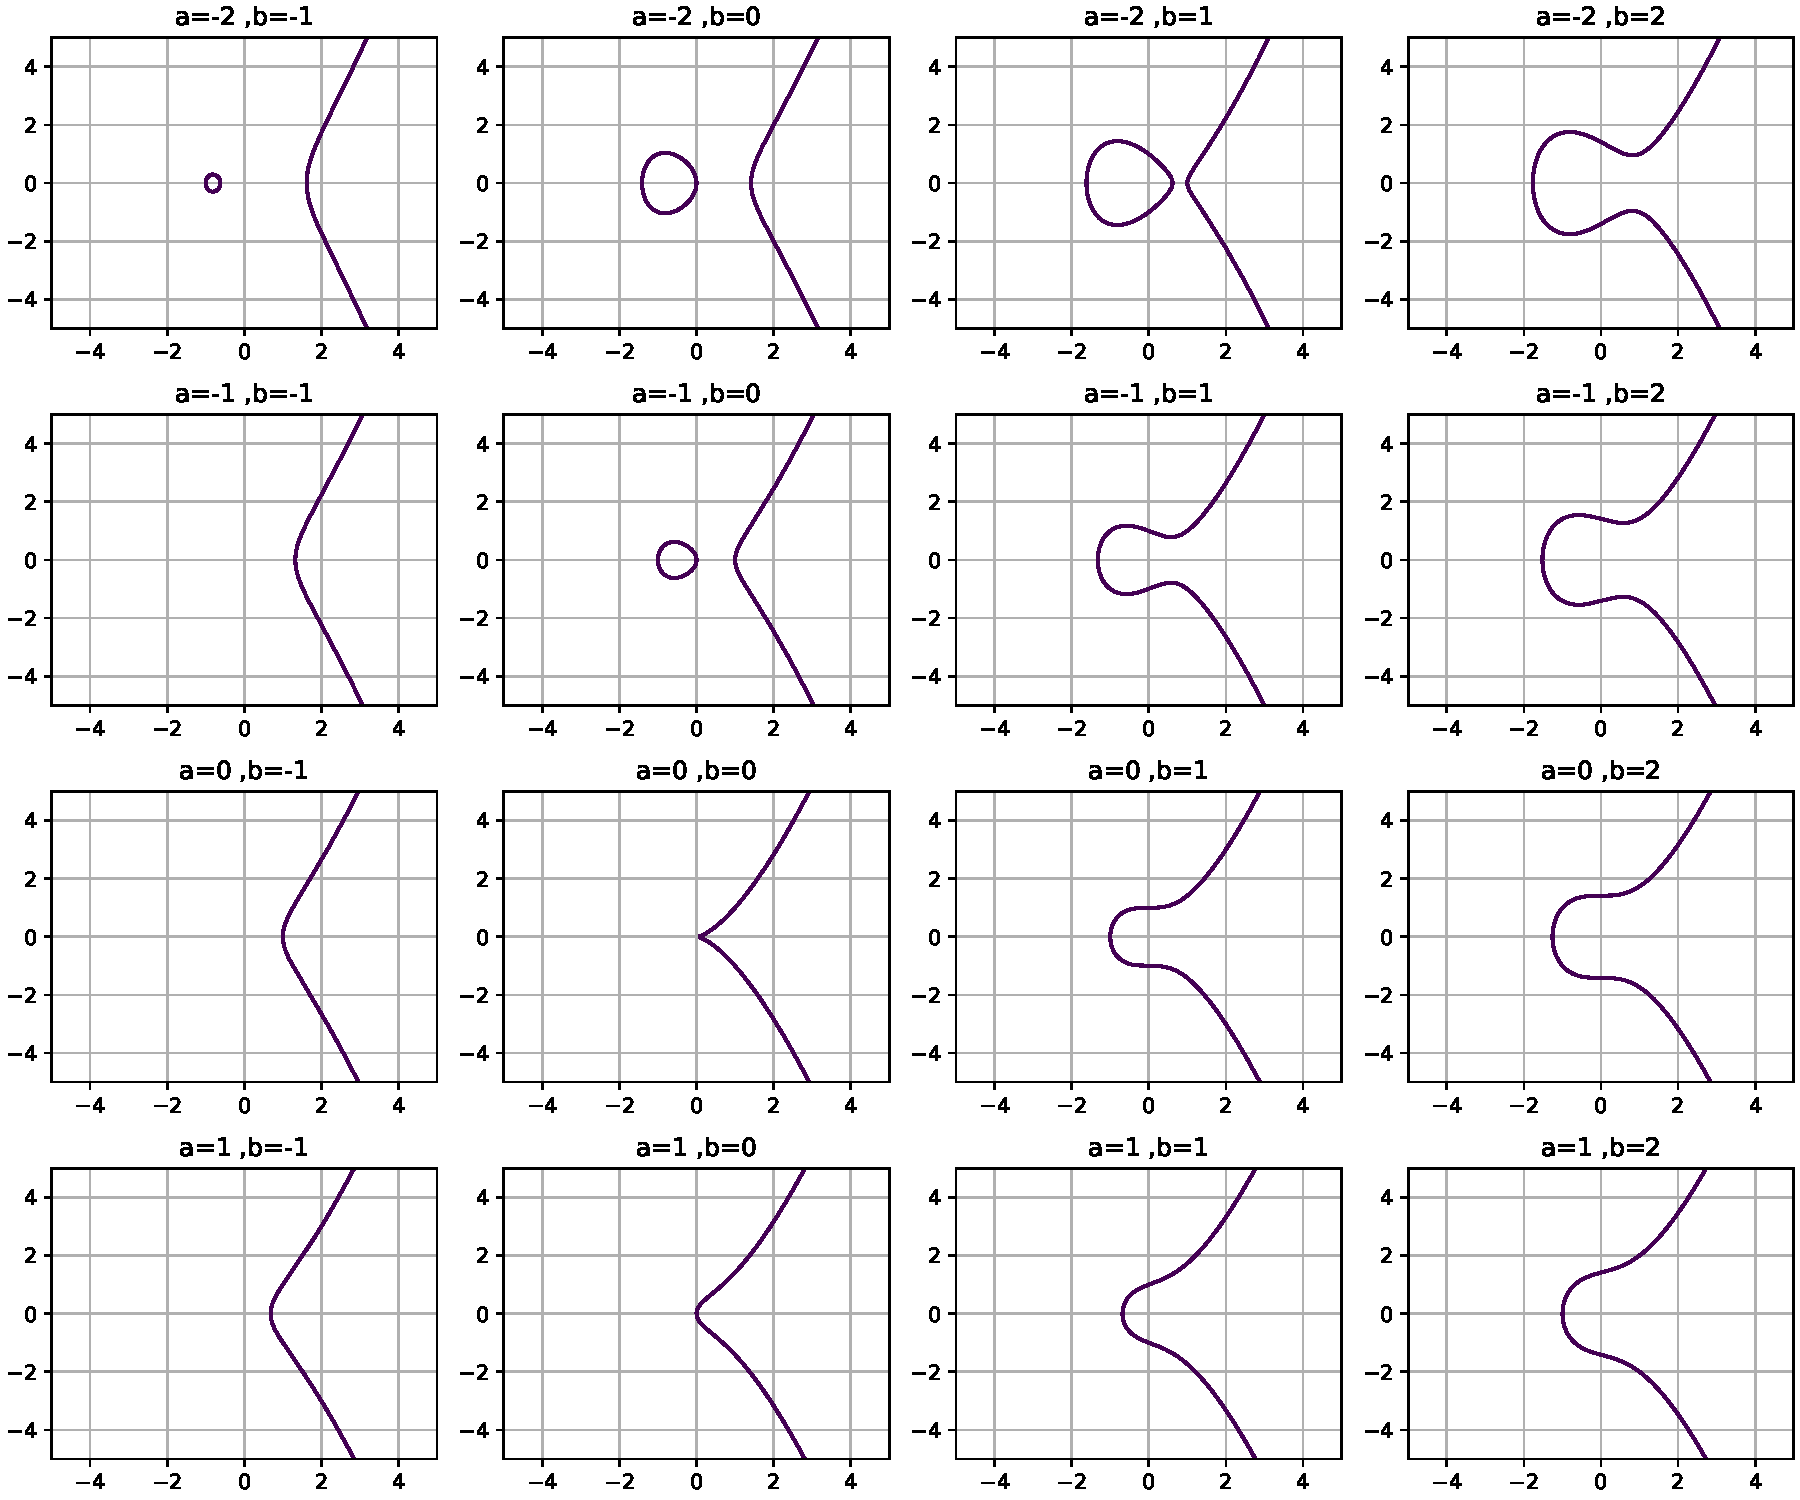
\includegraphics[width=1\linewidth]{./figure/elliptic_curves.pdf}
    \caption{Elliptic curves}
\end{figure}


\part{Mathematics}
% !TEX root = ../notes_template.tex
\chapter{Discrete Math}\label{chp:discrete_math}

\minitoc

gls examples:
\begin{itemize}
	% \item \glsxtrshort{gcd};
	\item \Gls{gcd}; \acrlong{gcd}; \acrshort{gcd}; \acrfull{gcd}
\end{itemize}

\section{Proof}
\begin{lemma}
\end{lemma}
\begin{claim}
\end{claim}
\begin{theorem}
\end{theorem}
\begin{example}
\end{example}
\begin{fact}
\end{fact}
\begin{remark}
\end{remark}
\begin{exercise}
	Prove A \iff B
\end{exercise}
\begin{solution}
By induction:
\end{solution}

\lipsum % dummy text - remove from real document

\section{Quantifier}
\lipsum % dummy text - remove from real document

\section{Graph}
\citetitle{babaiGraphIsomorphismQuasipolynomial2016}
\cite{babaiGraphIsomorphismQuasipolynomial2016}

\section{Number theory}
a Figure example
\begin{figure}[!ht]
    \centering
    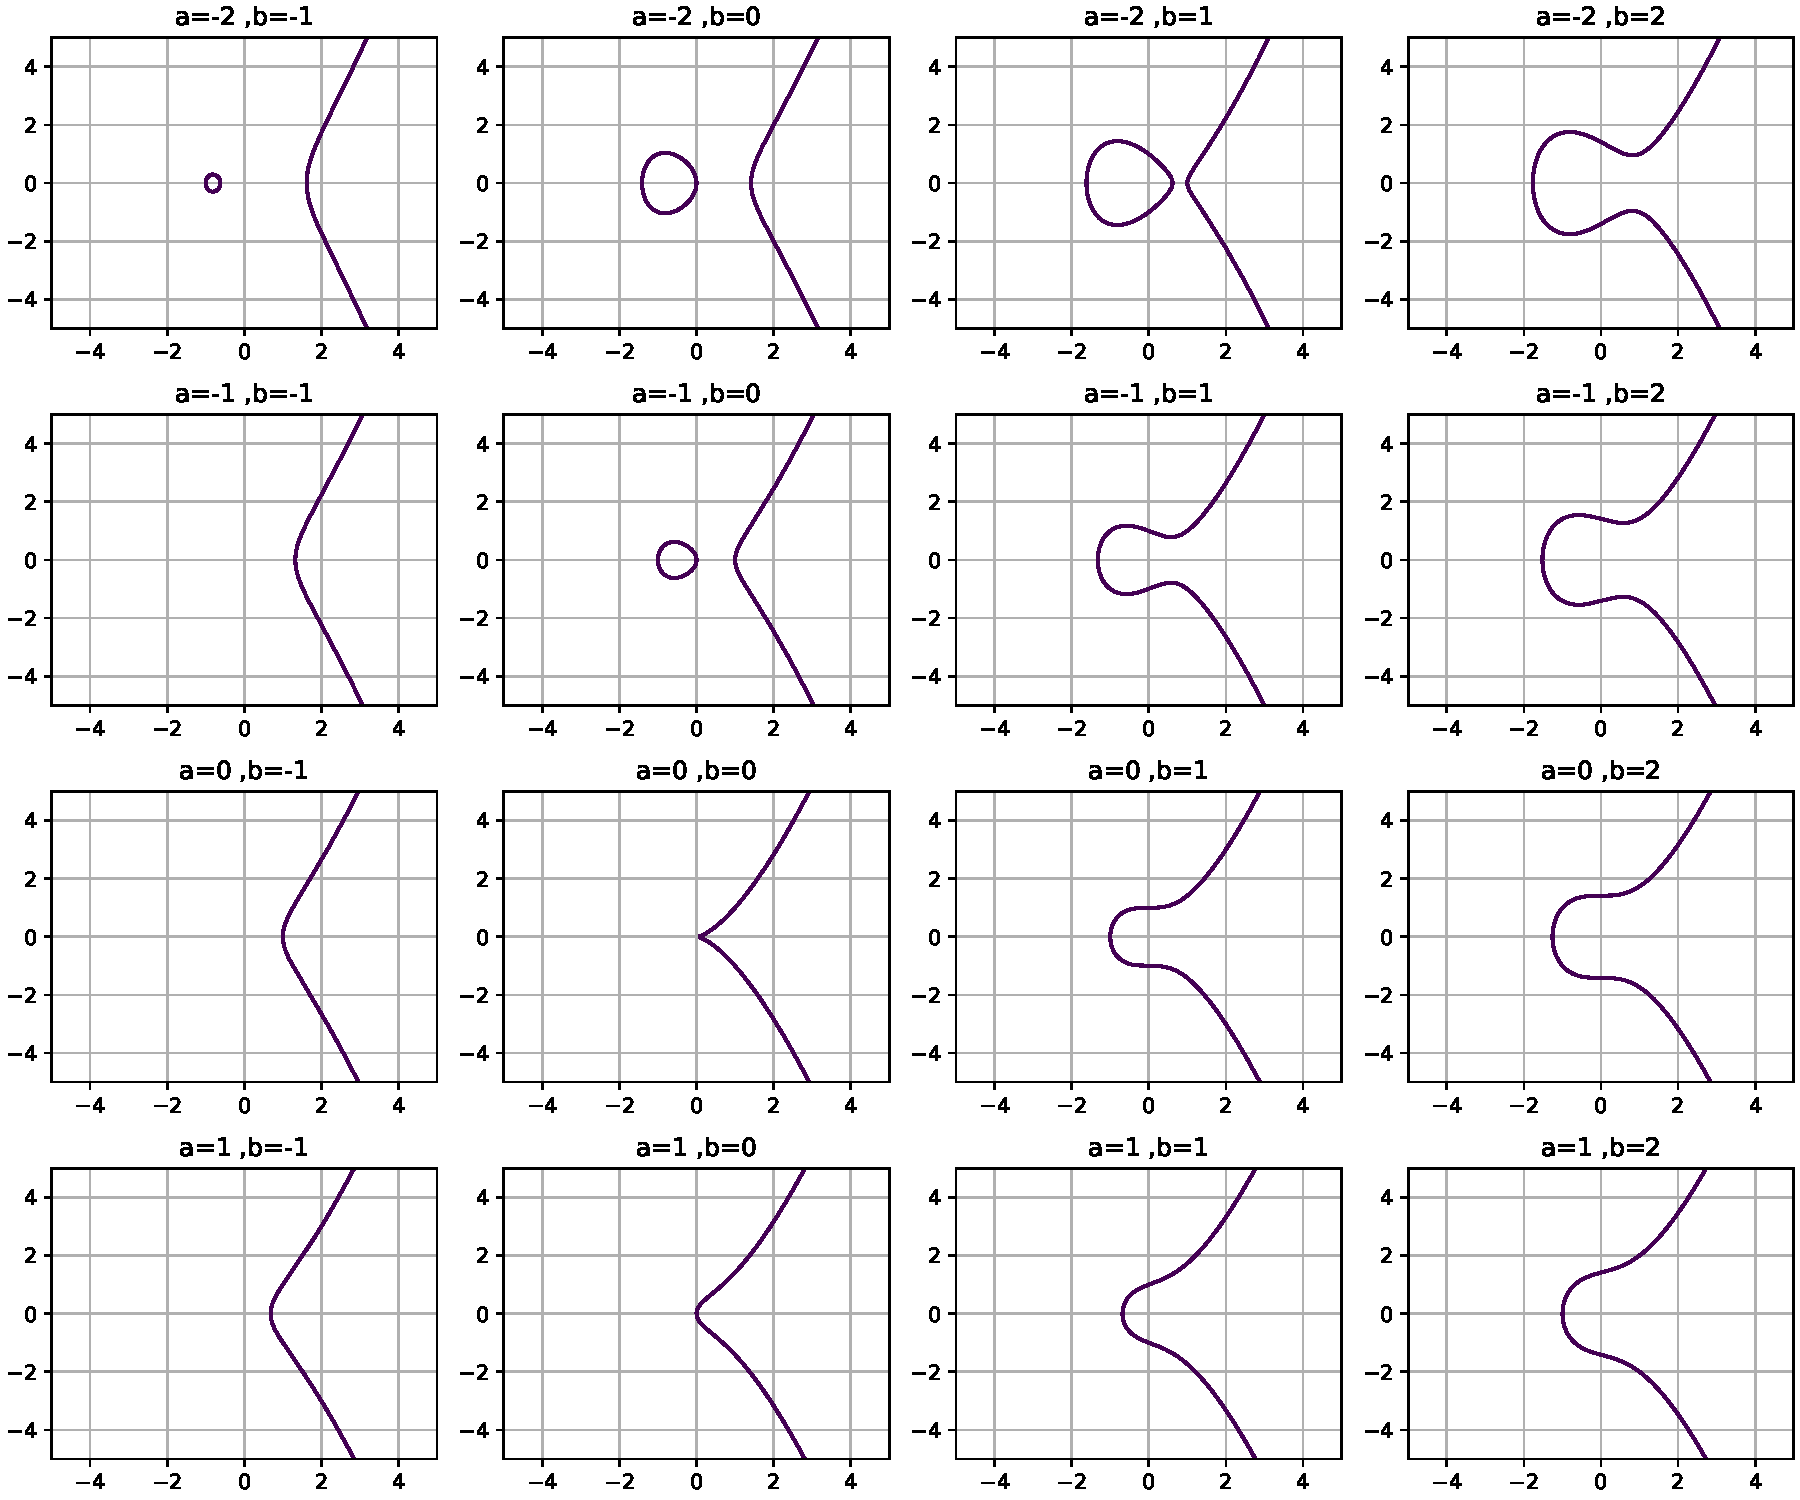
\includegraphics[width=1\linewidth]{./figure/elliptic_curves.pdf}
    \caption{Elliptic curves \cite{childsUniversalComputationQuantum2009} }
\end{figure}


\section{Algorithm}
% \begin{center}
% \begin{minipage}{.9\linewidth}
% algorithm2e
% https://www.overleaf.com/learn/latex/Algorithms#The_algorithm2e_package
\begin{algorithm}[H]
    \SetKwInOut{Input}{input}
    \SetKwInOut{Output}{output}
    \Input{Integer $N$ and parameter $1^t$}
    \Output{A decision as to whether $N$ is prime or composite}
    \BlankLine
    \For{ $i = 1,2, \ldots, t$} {
        $a\leftarrow \qty{1,\dots,N_1}$\;
        \If{$a^{N-1} \neq 1 \mod{N}$}
    {\Return "composite"}
    }
    \Return "prime"
    \caption{Primality testing - first attempt}
    \label{alg:miller_rabin}
\end{algorithm}
% \end{minipage}
% \end{center}

\part{Computer Science}
% \input{./chapter/complexity.tex}
% !TEX root = ../notes_template.tex
\chapter{Machine Learning}\label{chp:machine_learning}
\minitoc

\section{Regression}
% \gls{algorithm};
\subsection{Gradient descent}\label{sec:gradient_descent}
\gls{gd};
% \glsxtrshort{gd}

\section{Support Vector Machine}
\gls{svm};
% \input{./chapter/algorithms.tex}

\part{Physics}
% !TEX root = ../notes_template.tex
\chapter{Quantum Mechanics}\label{chp:quantum_mechanics}

\gls{hamiltonian};
\gls{qft};
\glsxtrshort{qm};
\gls{lagrangian}

% \input{./chapter/quantum_field_theory.tex}

\begin{appendices}
% !TEX root = ../notes_template.tex
\chapter{Formulas}

\section{Gaussian distribution}\label{sec:gaussian_distribution}
\begin{definition}[Gaussian distribution]\label{def:gaussian_distribution}
    \myindex{Gaussian distribution}
\end{definition}

\begin{theorem}[Central limit theorem]\label{thm:central_limit_theorem}
\end{theorem}
\end{appendices}

\backmatter

%%%%%%%%%%%%%%% Reference %%%%%%%%%%%%%%%

\printbibliography[heading=bibintoc]
\printindex

\end{document}

